\chapter{The Fundamental Theorem of Calculus}

The Fundamental Theorem of Calculus (FTC) is a theorem that connects the
concept of differentiating a function with the concept of integrating
a function. This theorem is divided into two parts:\index{fundamental theorem of calculus}

\section{First Part}

The first part of the Fundamental Theorem of Calculus states that if
$f$ is a continuous real-valued function defined on a closed interval
$[a, b]$ and $F$ is the function defined, for all $x$ in $[a, b]$, by:

\begin{equation}
F(x) = \int_a^x f(t) \, dt
\end{equation}

Then, $F$ is uniformly continuous and differentiable on the open
interval $(a, b)$, and $F'(x) = f(x)$ for all $x$ in $(a, b)$.
(That is $F(x)$ is the antiderivative of $f(x)$.)

\section{Second Part}

The second part of the Fundamental Theorem of Calculus states that if
$f$ is a real-valued function defined on a closed interval $[a, b]$
that admits an antiderivative $F$ on $[a, b]$, and $f$ is integrable
on $[a, b]$ (it need not be continuous), then

\begin{equation}
\int_a^b f(t) \, dt = F(b) - F(a).
\end{equation}

We will also use shorthand as follows:

\begin{equation}
\int_a^b f(t)\,dt = F(t)|_a^b
\end{equation}

Which means "$F(t)$ evaluated from $t=a$ to $t=b$". 

\section{The Meaning of the FTC}
What the Fundamental Theorem of Calculus is really saying is that 
differentiation and integration are opposite processes. Mathematically, 
we can say $$\frac{d}{dx} \int_{a}^{x} f(t)\,dt = f(x)$$
This may seem clunky, but many useful functions are defined this way. 
Consider the Fresnel function, $S(x) = \int_{0}^{x}\sin{
\frac{\pi t^2}{2}}\,dt$. Originally used in optics, this equation is 
also used by civil engineers to design road and railway curves. 
According to FTC, then, $S'(x) = \sin{\frac{\pi t^2}{2}}$. 

We can also apply the Chain Rule when taking derivatives of integrals. 
Let $f(x) = \int_{1}^{x^4} \sec{t}\,dt$. What is $f'(x)$? First, let 
us define $u = x^4$. By the Chain Rule,
$$\frac{d}{dx}\int_{0}^{x^4} \sec{t}\,dt = \frac{d}{dx}\int_{0}^{u} 
\sec{t}\,dt$$ 
$$= \frac{d}{du}[\int_{0}^{u} \sec{t}\,dt]\frac{du}{dx}$$
$$ = \sec{u} \frac{du}{dx}$$
Noting that $\frac{du}{dx} = \frac{d}{dx}x^4 = 4x^3$, 
$$f'(x) = \sec{x^4}(4x^3)$$

\subsection{FTC Practice}
\begin{Exercise}[label=FTC1]
Use the Fundamental Theorem of Calculus to find the derivative of the 
function. 
	\begin{enumerate}
	\item $g(x) = \int_0^x \sqrt{t + t^3}\,dt$
	\item $F(x) = \int_x^0 \sqrt{1 + \sec{t}}\,dt$
	\item $h(x) = \int_1^{e^x} \ln{t}\,dt$
	\item $y = \int_{\sqrt{x}}^{\frac{\pi}{4}} \theta \tan{\theta}\,
	d\theta$
	\end{enumerate}
\end{Exercise}

\begin{Answer}[ref=FTC1]
	\begin{enumerate}
	\item $g'(x) = \sqrt{x + x^3}$
	\item $F(x) = - \int_0^x \sqrt{1+\sec{t}}\,dt$ and therefore $F'(x) = 
	- \sqrt{1+\sec{x}}$
	\item setting $u = e^x$ and noting $\frac{du}{dx} = e^x$, then $h'(x) 
	= \frac{d}{du}\int_1^{u} \ln{t}\,dt(\frac{du}{dx})$ Taking the 
	derivative and substituting for $\frac{du}{dx}$, we find $h'(x) = 
	\ln{u} \cdot e^x = \ln{(e^x)} \cdot e^x = x \cdot e^x$
	\item $y = - \int_{\frac{\pi}{4}}^{\sqrt{x}} \theta \tan{\theta}\,
	d\theta$. Setting $u = \sqrt{x}$ and noting that $\frac{du}{dx} = 
	\frac{1}{2\sqrt{x}}$, we see that $y' = -\frac{d}{du}
	[\int_{\frac{\pi}{4}}^{u}\theta\tan{\theta}\,d\theta]\frac{du}{dx} 
	= u\tan{u} \cdot \frac{1}{2\sqrt{x}} = -\sqrt{x}\tan{\sqrt{x}} \cdot 
	\frac{1}{2\sqrt{x}} = \frac{-\sqrt{x}\tan{\sqrt{x}}}{2\sqrt{x}} = 
	- \frac{1}{2}\tan{\sqrt{x}}$
	\end{enumerate}
\end{Answer}

\section{Using Antiderivatives to Evaluate Definite Integrals}
In everyday English, the FTC states that the integral from $a$ to $b$ 
of a function is the antiderivative of that function evaluated from 
$a$ to $b$. In the previous chapter, the integrals presented were of 
linear functions where the area under the curve could be equally 
calculated by hand. The FTC connects integrals to antiderivatives, 
allowing us to evaluate more complex integrals. Consider the following 
example:\\

The power consumption of a household can be modeled as 
$P(t) = \frac{1}{10} t^2 (t - 24)^2$ from $t = 0$ to $t = 24$, where 
$P$ is measured in watts and $t$ is measured in hours ($t = 0$ is 
midnight). The total energy the household uses is given by $\int_{0}^{24} 
P(t)\,dt$. As you can see from the graph (see figure \ref{fig:power}), 
we cannot simply use our geometry skills to determine the area under 
the curve. 

\begin{figure}
	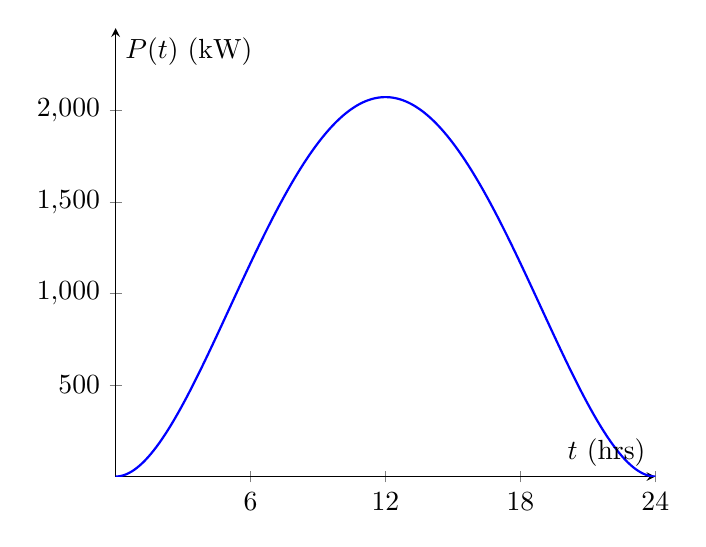
\begin{tikzpicture}
		\begin{axis}
		[axis lines = center, xmin = 0, xmax = 24, xlabel = $t$ (hrs),
		ymin = 0, ymax = 2450, ylabel = $P(t)$ (kW),
            xtick={6, 12, 18, 24}]
		\addplot[blue, thick, samples=200, domain =0:24] {0.1*x^2*(x-24)^2};
		\end{axis}
	\end{tikzpicture}
	\caption{Power consumption of a household in a day}
	\label{fig:power}
\end{figure}

To determine the total energy use, we need to evaluate $\int_{0}^{24} 
\frac{1}{10}t^2(t-24)^2\,dt$. First, we expand the polynomial:\\
$$E_{tot} = \frac{1}{10} \int_{0}^{24} t^2 (t^2-48t+576)\,dt = 
\frac{1}{10}\int_{0}^{24} t^4 - 48t^3 + 576t^2\,dt$$
$$= \frac{1}{10}\int_{0}^{24} t^4\,dt - \frac{24}{5}\int_{0}^{24} 
t^3\,dt + \frac{288}{5}\int_{0}^{24} t^2\,dt$$\\
Using the Power Rule to determine the antiderivatives of $t^4$, $t^3$, 
and $t^2$, we see:\\
$$=\frac{1}{10}[\frac{1}{5}t^5]|_{0}^{24} - \frac{24}{5}
[\frac{1}{4}t^4]|_{0}^{24} + \frac{288}{5}[\frac{1}{3}t^3]|_{0}^{24} 
= 26542.1 Whr = 26.5421 kWhr$$

\subsection{Definite Integrals Practice}
\begin{Exercise}[label=FTC2]
	Evaluate the following integrals:
	\begin{enumerate}
	\item $\int_1^4 t^{-3/2}\,dt$
	\end{enumerate}
\end{Exercise}

\begin{Answer}[ref=FTC2]
	\begin{enumerate}
	\item The antiderivative of $t^{-3/2}$ is $\frac{-2}{\sqrt{t}}$. 
	Therefore, the integral is equal to $[\frac{-2}{\sqrt{t}}]_1^4 = 
	\frac{-2}{\sqrt{4}} - \frac{-2}{\sqrt{1}} = -1 + 2 = 1$. 
	\end{enumerate}
\end{Answer}

\begin{Exercise}[label=FTC3]
	[This question was originally presented as a multiple-choice, 
	no-calculator problem on the 2p Calculus BC exam.] The graph of a 
	differentiable function $f$ is shown in the graph. $h(x) = \int_0^x 
	f(t)\,dt$. Rank the relative values of $h(6)$, $h'(6)$, and $h''(6)$ 
	from lowest to highest.
	
	\begin{tikzpicture}
		\begin{axis}
		[axis lines = center, xlabel = $x$, ylabel = $f(x)$,
		xmin = 0, xmax = 9, xtick = {1, 2, 3, 4, 5, 6, 7, 8, 9},
		ymin = -4, ymax = 2, ytick = {-4, -3, -2, -1, 1, 2}]
		\addplot[blue, thick, samples=100, domain = 0:9]
		{2.5*sin(30*(x+6.6))-0.75};
		\end{axis}
	\end{tikzpicture}
\end{Exercise}

\begin{Answer}[ref=FTC3]
According to FTC, $h'(x) = f(x)$ and $h''(x) = f'(x)$. Examining the 
graph, we see that the curve lies below the $x$-axis for $0<x<6$, 
which means that $h(6) = \int_0^6 f(t)\,dt < 0$. $h'(6) = f(6) = 0$ 
and $h''(6) = f'(6) > 0$. Therefore, $h(6) < h'(6) < h''(6)$. 
\end{Answer}

\begin{Exercise}[label=defint6]
	The graph of $f'$ is shown in the graph and consists of a semi-circle 
	and two line segments. If $f(2) = 1$, then what is $f(-5)$?\\
	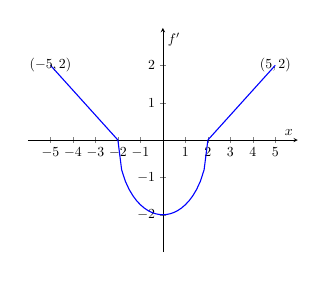
\begin{tikzpicture}[scale = 0.5]
		\begin{axis}
		[axis lines = center, xmin = -6, xmax = 6, xlabel = $x$,
		xtick = {-5, -4, -3, -2, -1, 1, 2, 3, 4, 5},
		ymin = -3, ymax = 3, ylabel = $f'$, ytick = {-2, -1, 2, 1}]
		\addplot[blue, thick]coordinates{(-5, 2) (-2, 0)};
		\node[] at (5, 2) {$(5, 2)$};
		\node[] at (-5, 2) {$(-5, 2)$};
		\addplot[blue, thick]coordinates{(5, 2) (2, 0)};
		\addplot[blue, thick, domain = -2:2]{- sqrt(4 - x^2)};
		\end{axis}
	\end{tikzpicture}
\end{Exercise}

\begin{Answer}[ref=defint6]
	We know that $f(2) = \int_{-5}^2 f'(x)\,dx + f(-5)$. Examining the 
	graph, we know that $\int_{-5}^2 f'(x)\,dx = frac{1}{2}(3)(2) - 
	\frac{1}{2}\pi(2^2)$ (the area of the triangle above the $x$-axis 
	less the area of the semi-circle below the axis). Therefore, $f(-5) 
	= f(2) - \int_{-5}^2 f'(x)\,dx = 1-(3-2\pi) = 2\pi-2$
\end{Answer}



